\section{\ce{[Cu(SCN)_2(4-hydroxymethylpyridine)_2]_2}}
\subsection{Synthesis}
0.48 g \ce{Cu(NO_3)_2* 3 H_2O} (2 mmol), 0.39 g KSCN (4 mmol) and 0.44 g 4-hydroxymethyl-pyridine (4 mmol) were dissolved in 35 mL distilled \ce{H_2O}. The solution was heated up to 70$^\circ$C  and stirred for 2 hours. After filtration the green solution was stirred again for 20 minutes at the same temperature and then cooled down to RT. After a few hours small green crystals were obtained.
Anal. Calculated for \ce{C_{28}H_{28}Cu_{2}N_{8}O_{4}S_4} (795.92 g/mol) : 42.25\% C; 3.55\% H; 14.08\% N; 16.11\% S;
Found: 42.19 \% C; 3.58\% H; 14.15 \% N; 15.60\% S;
IR (ATR, cm$^{-1}$): 3456 (w), 3275 (m), 2093 (s), 1616 (m), 1561 (w), 1504 (w), 1423 (s), 1365 (m), 1195 (w), 1101 (vw), 1050 (m), 1019 (s), 801 (vs), 743 (w), 714 (w), 665 (w), 610 (m), 513 (w), 490 (m), 462 (m)

\begin{figure}[h!]
\centering
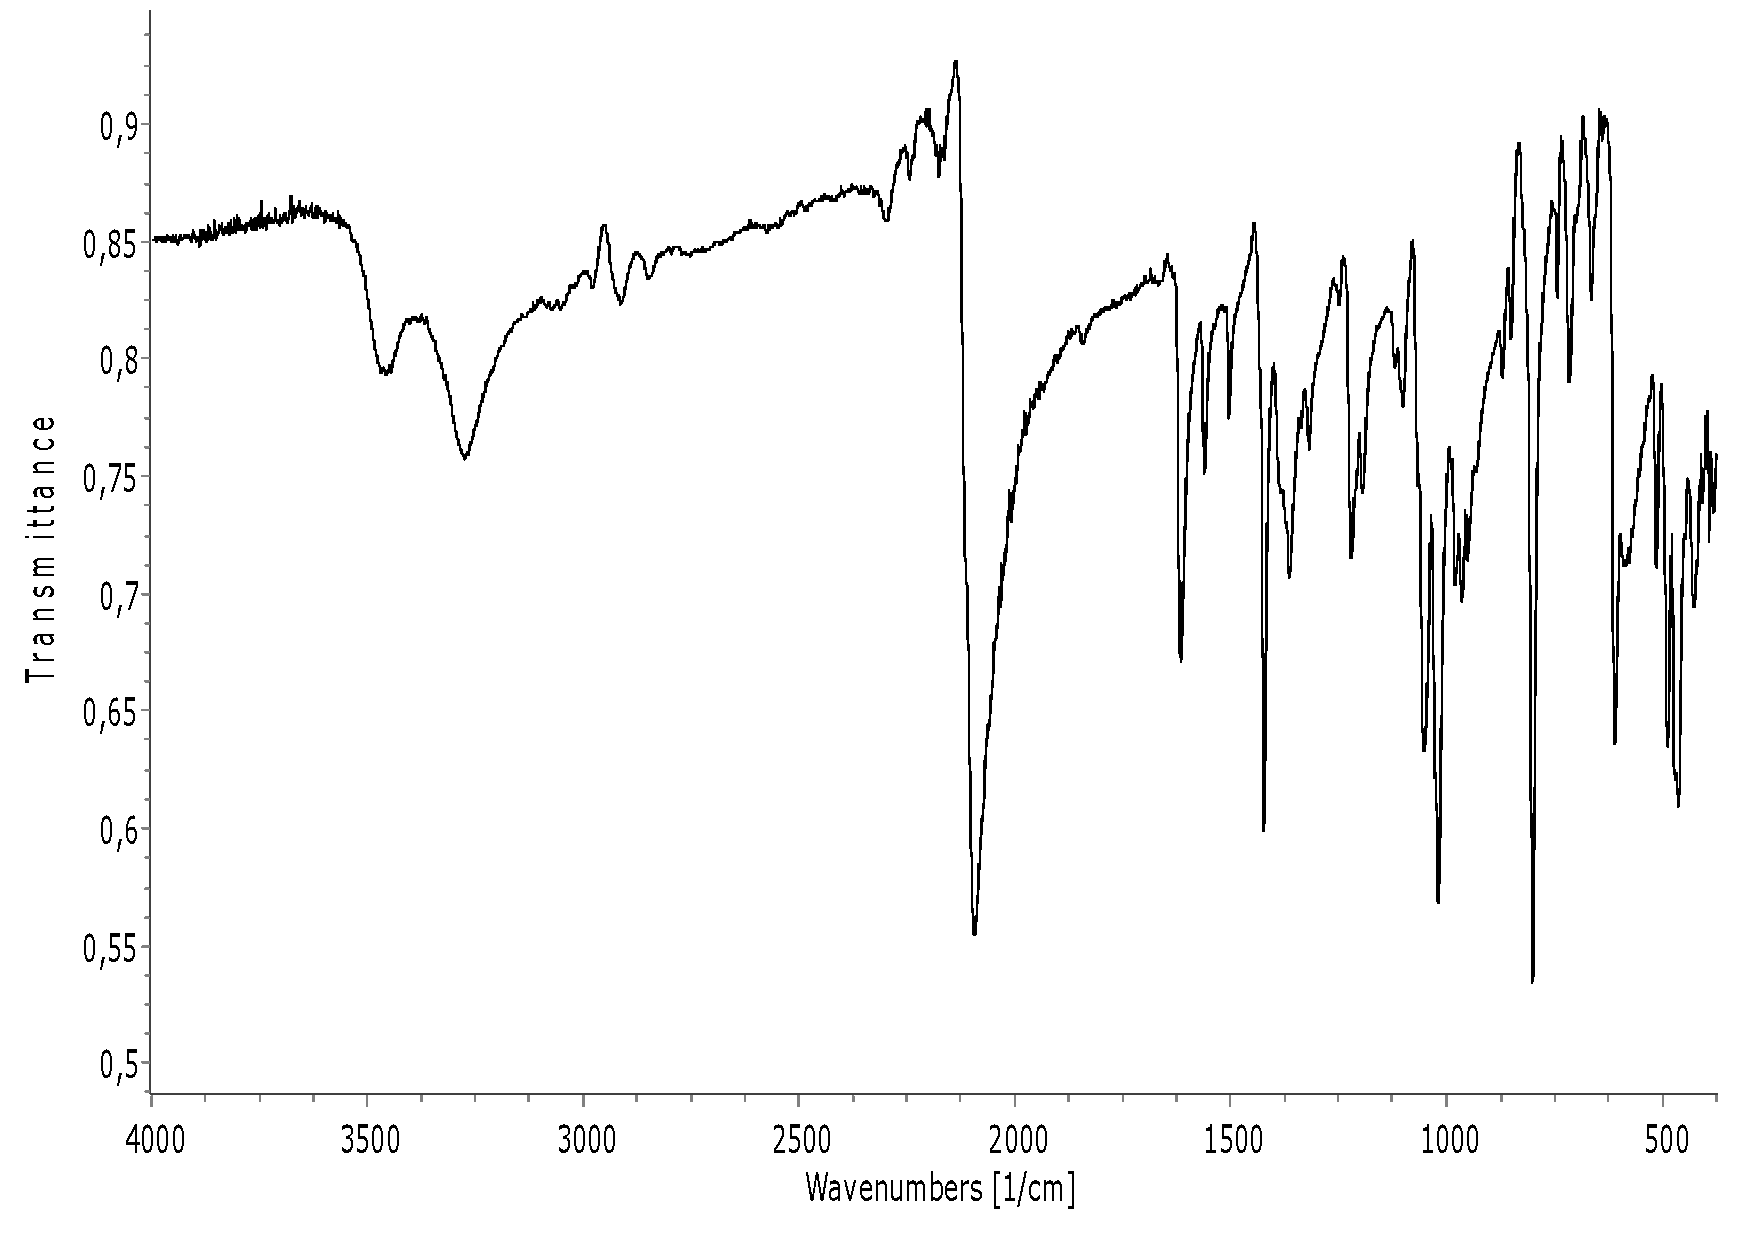
\includegraphics[width=1\textwidth]{figures/CuR4HOMP-IR.pdf}
\caption{IR spectrum of \ce{[Cu(SCN)_2(4-HOMepy)_2]_2}}
\end{figure}

\newpage
\subsection{Structural characterization}

A perspective view of \ce{[Cu(SCN)_2(4-HOMepy)_2]_2} is given in fig. \ref{fig:CuR4HOMP_pv} and a packing view in fig. \ref{fig:CuR4HOMP_packv}. Table \ref{batlb:CuR4HOMP} lists the selected bond parameters. The Cu(1) metal center is penta-coordinated by N(1) and N(2) atoms of two terminal isothiocyanato anions, by N(3) of a terminal 4-hydroxymethylpyridine molecule and further by O(2) and N(4’) atoms of two $\mu$ (N,O)-bridging  4-hydroxymethylpyridine molecules. The latter connect Cu(1) and Cu(1’) polyhedra to form centrosymmetric dinuclear units. The \ce{CuN4O} chromophore may be described as slightly distorted square pyramid (SP) with a $\tau$-value of 0.03 ($\tau$-values of 1 and 0 refer to ideal geometries of trigonal bipyramid (TBP) and square pyramid (SP), respectively) \cite{addison}. The apical site is occupied by O(2) [Cu(1)-O(2) = 2.379(4) \AA]. The basal Cu-N bond distances are in the range of 1.954(4) to 2.041(4) \AA. The terminal isothiocyanate anions possess the following bond parameters: N-C: 1.138(6) and 1.156(6) \AA, C-S: 1.644(4) and 1.637(4) \AA, Cu-N-C: 170.8(4) and 169.0(4)$^\circ$, N-C-S: 178.0(5 and 178.7(4)$^\circ$. The Cu(1)\ce{***}Cu(1’) distance is 7.9083(14) \AA \ \ and the shortest inter-dinuclear metal-metal separation is 5.8666(12) \AA. Along the c-axis the Cu(1)\ce{***}S(2c) separation is 3.1172(16) \AA. Hydrogen bonds of type O-H\ce{***}S between hydroxy-groups of pyridine derivative ligands and adjacent non-coordinated S atoms of terminal isothiocyanate anions form a supramolecular 2D system oriented along the b- and c-axis of the monoclinic unit cell (O(1)-H(91)\ce{***}S(2\#1) = 155(3)$^\circ$, O(1)\ce{***}S(2\#1) = 3.454(4) \AA; O(2)-H(92)\ce{***}S(1\#2) = 172(3)$^\circ$, O(2)\ce{***}S(1\#2) = 3.168(3) \AA; (\#1): x,1/2-y,1/2+z; (\#2): x,1/2-y,-1/2+z ). \ce{Cu(SCN)_2(4-HOMepy)_2} is isostructural to the corresponding Co(II) complex.


\begin{table}
\centering
\captionabove{Selected bond lengths (\AA) and angles ($^\circ$) for \ce{[Cu(SCN)_2(4-HOMepy)_2]_2}.}
\begin{tabular}{|l|l|l|l|}
\hline
Cu(1)-N(1) & 1.973(4) & Cu(1)-N(4') & 2.041(4)\\
\hline
Cu(1)-N(2) & 1.954(4) & Cu(1)-O(2) & 2.379(4)\\
\hline
Cu(1)-N(3) & 2.028(4) & S(1)-C(1) & 1.644(4)\\
\hline
N(1)-C(1) & 1.138(6) & S(2)-C(2) & 1.637(5)\\
\hline
N(2)-C(2) & 1.156(6) &  & \\
\hline
\hline
N(2)-Cu(1)-N(1) & 177.58(18) & N(2)-Cu(1)-N(3) & 88.83(16)\\
\hline
N(1)-Cu(1)-N(3) & 88.87(16) & N(2)-Cu(1)-N(4') & 91.78(16)\\
\hline
N(1)-Cu(1)-N(4') & 90.52(16) & N(3)-Cu(1)-N(4') & 179.39(16)\\
\hline
N(2)-Cu(1)-O(2) & 93.01(15) & N(1)-Cu(1)-O(2) & 87.81(15)\\
\hline
N(3)-Cu(1)-O(2) & 92.30(14) &N(4)-Cu(1)-O(2') & 87.69(15)\\
\hline
Cu(1)-N(1)-C(1) & 170.8(4) & N(1)-C(1)-S(1) & 178.0(5)\\
\hline
Cu(1)-N(2)-C(2) & 169.0(4) & N(2)-C(2)-S(2) & 178.7(4)\\
\hline
\end{tabular}
\label{batlb:CuR4HOMP}
\end{table}






\begin{figure}[!htpb]
\centering
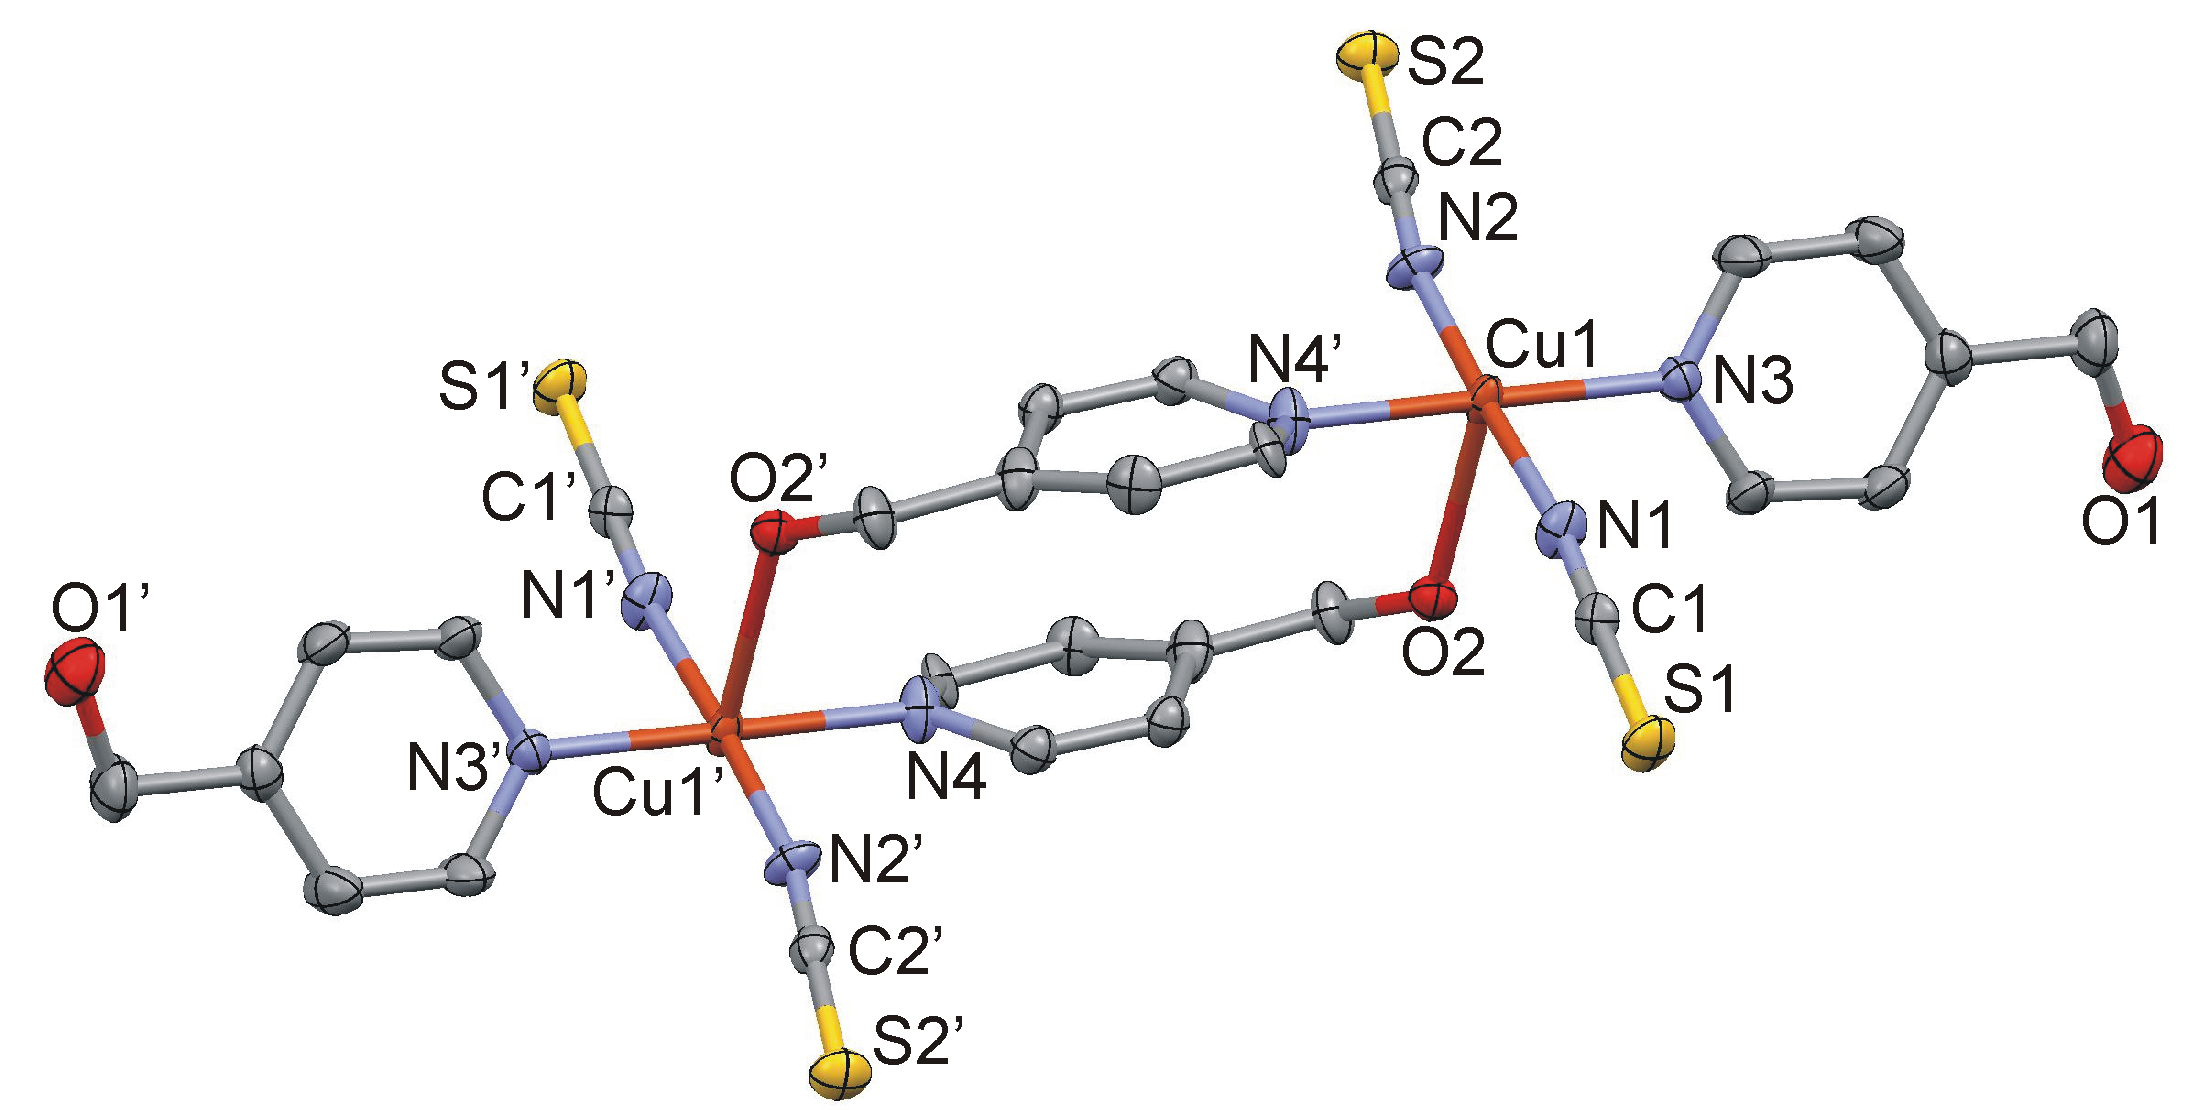
\includegraphics[width=1\textwidth]{figures/curhomp_FIGm11.png}
\caption[Perspective view of \ce{[Cu(SCN)_2(4-HOMepy)_2]_2}]{Perspective view of \ce{[Cu(SCN)_2(4-HOMepy)_2]_2} with the atom numbering scheme. Symmetry codes:(‘) 1-x,1-y,1-z.}
\label{fig:CuR4HOMP_pv}
\vspace{\floatsep}
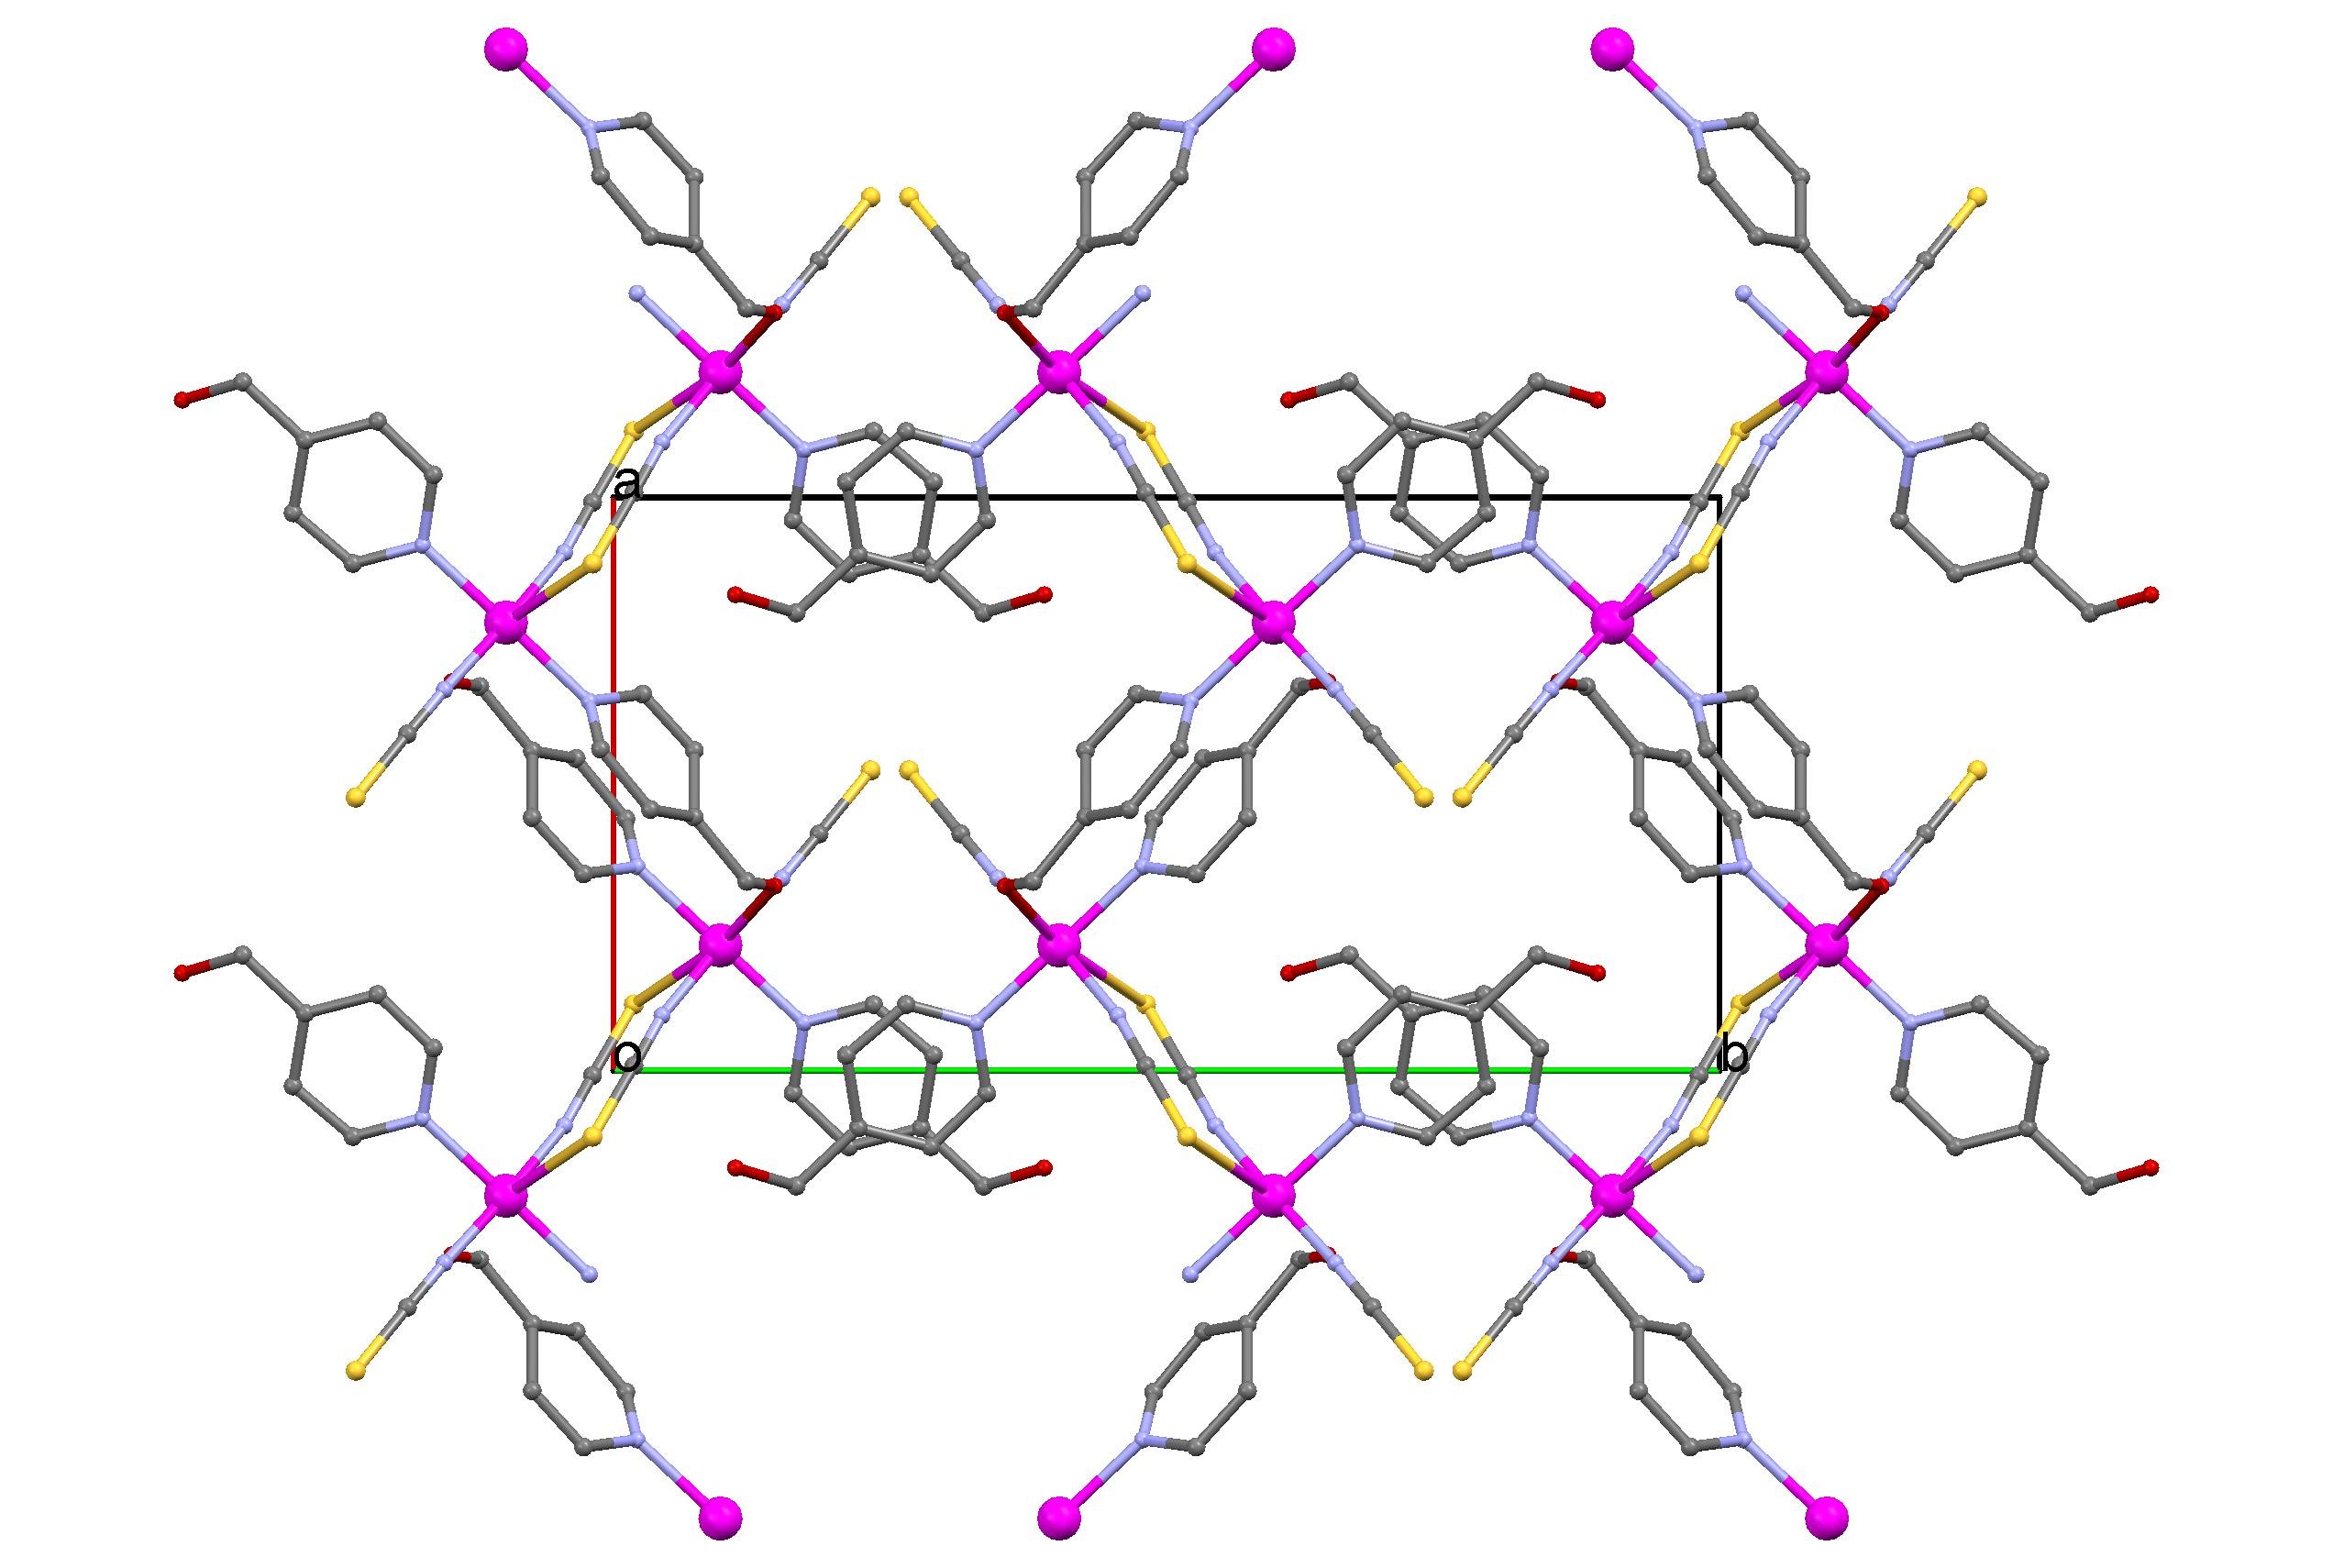
\includegraphics[width=1\textwidth]{figures/curhomp_CC.png}
\caption{Packing plot of \ce{[Cu(SCN)_2(4-HOMepy)_2]_2}.}
\label{fig:CuR4HOMP_packv}
\end{figure}



\renewcommand{\arraystretch}{1.5}

\begin{table}
\captionabove{Crystallographic data and processing parameter of \ce{[Cu(SCN)_2(4-HOMepy)_2]2}}
\centering
\begin{tabular}{ | l |  l | }
\hline
Empirical formula & \ce{C_{28}H_{28}Cu_{2}N_{8}O_{4}S_4}\\
\hline
Formula mass & 795.92\\
\hline
System & monoclinic\\
\hline
Space group & P2$_{1}$/c\\
\hline
a ({\AA}) & 10.9582(14)\\
\hline
b ({\AA}) & 19.6859(18)\\
\hline
c ({\AA}) & 8.0786(12)\\
\hline
$\alpha$ ($^\circ$) & 90\\
\hline
$\beta$ ($^\circ$) & 111.469(2)\\
\hline
$\gamma$ ($^\circ$) & 90\\
\hline
V (\AA$^{3}) $  & 1621.8(4)\\
\hline
Z & 2\\
\hline
T (K) & 100(2)\\
\hline
$\mu$ (mm$^{-1}$) & 1.617\\
\hline
 D$_{calc}$ (Mg/m$^{3}$) & 1.630\\
\hline
Crystal size (mm) & 0.26 x 0.20 x 0.13\\
\hline
$\theta$ max ($^\circ$) & 25.28\\
\hline
Data collected & 11792\\
\hline
Unique refl./ R$_{int}$ & 2934 / 0.0714\\
\hline
Parameters & 250\\
\hline
Goodness-of-Fit on F$^{2}$ & 1.360\\
\hline
R1 / wR2 (all data) & 0.0880 /0.1735\\
\hline
Residual extrema (e/\AA$^{3}$) & 0.99 /-0.73\\
\hline
\end{tabular}

\label{ptab:CuR4HOMP}

\end{table}

